\documentclass[tikz,border=8pt]{standalone}
\usepackage{pgfplots}
\pgfplotsset{compat=1.18}
\begin{document}
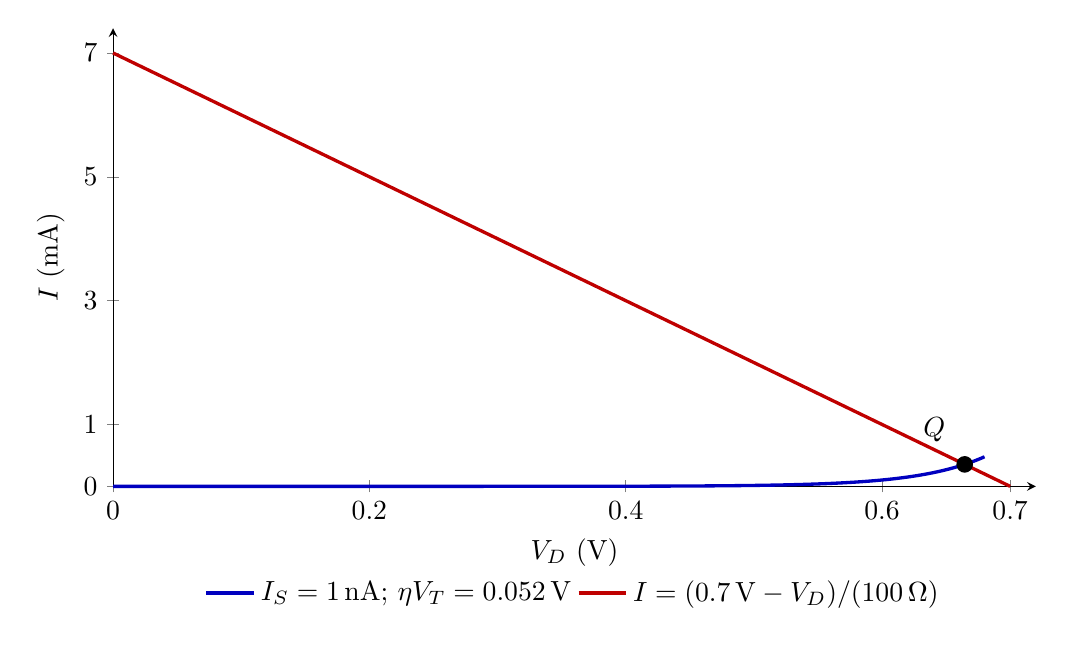
\begin{tikzpicture}
\begin{axis}[
  width=13.3cm,height=7.4cm,
  xmin=0,xmax=0.72,ymin=0,ymax=7.4,
  axis lines=left,xlabel={$V_D$ (V)},ylabel={$I$ (mA)},
  xtick={0,0.2,0.4,0.6,0.7},ytick={0,1,3,5,7},clip=false,
  legend style={at={(0.5,-0.18)},anchor=north,legend columns=2,draw=none}
]
\addplot[very thick,blue!75!black,domain=0:0.68,samples=300]{1e-6*(exp(x/0.052)-1)};
\addlegendentry{$I_S=1\,\mathrm{nA}$; $\eta V_T=0.052\,\mathrm V$}
\addplot[very thick,red!75!black,domain=0:0.7,samples=2]{10*(0.7-x)};
\addlegendentry{$I=(0.7\,\mathrm V-V_D)/(100\,\Omega)$}
\addplot[only marks,mark=*,mark size=2.8pt,black] coordinates {(0.664522,0.354783)};
\node[anchor=south east] at (axis cs:0.657,0.56) {$Q$};
\end{axis}
\end{tikzpicture}
\end{document}
